\subsection{Launcher}\label{sec:launcher}
A launcher in Android terminology is an application that provides easy access to other applications present in the system.
When the system is fully booted, the launcher is automatically started and thus is comparable to booting a desktop computer directly to the desktop.

From this point and onwards, when referring to \launcher, we are drawing attention to the launcher that is part of the \giraf application suite.

The main purpose of \launcher is to provide a user-friendly means of accessing other applications in the \giraf suite, as well as regulating access to these based on the active user profile.

\subsubsection{Motivation for Working with Launcher}
\launcher was originally developed by \citet{launcher2011}, and further refined by \citet{launcher2012}.
At an introductory meeting with the clients however, they made us aware that \launcher is rarely used, as it often crashes.
They preferred to access the \giraf applications through the Android native launcher.
As mentioned in \cref{sec:sprint1:objectives}, the focus in this sprint is on creating running applications, and since \launcher was relatively complete based on the development of \citet{launcher2012}, but reported as being unreliable by the clients, an obvious task for this sprint is to make \launcher run reliably.

\subsubsection{Launcher Functionality}
As the \launcher covers multiple tasks in the \giraf project, this section gives a detailed description of its most important activities.
Screenshots of each activity is found in \cref{fig:launcheractivities}.

\begin{figure}[h] % Billeder af draweren i åben og lukket tilstand
\centering
	\begin{subfigure}[b]{.48\textwidth}
	\centering
	
\includegraphics[width=\textwidth, height=3in, keepaspectratio=true] {screenshots-old-giraf/giraf-logoactivity.png}
	\caption{\mainactivity.}
	\label{fig:launcheractivity:logo}
	\end{subfigure}
	\hfill
	\begin{subfigure}[b]{.48\textwidth}
	\centering
	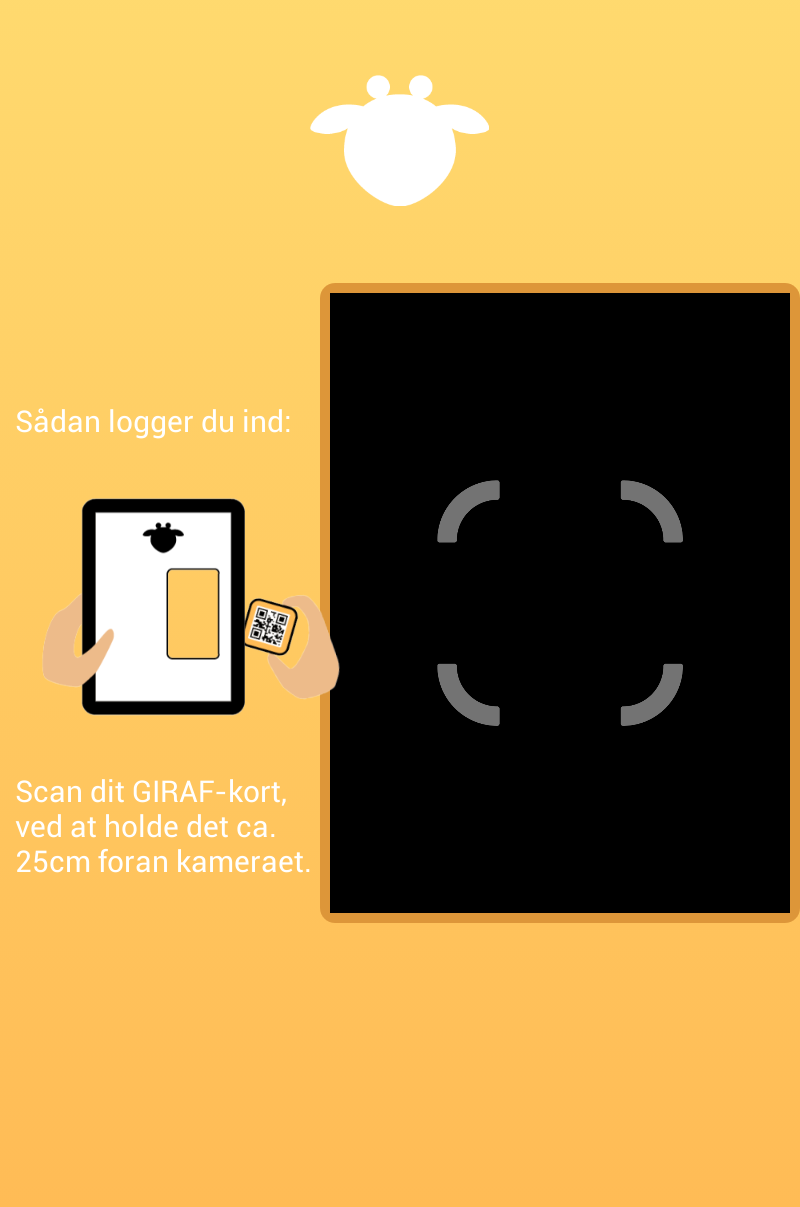
\includegraphics[width=\textwidth, height=3in, keepaspectratio=true] {screenshots-old-giraf/giraf-authenticationactivity.png}
	\caption{\authenticationactivity.}
	\label{fig:launcheractivity:auth}
	\end{subfigure}
	
	\quad % Inserts extra space between rows of subfigures
	
	\begin{subfigure}[b]{.48\textwidth}
	\centering
	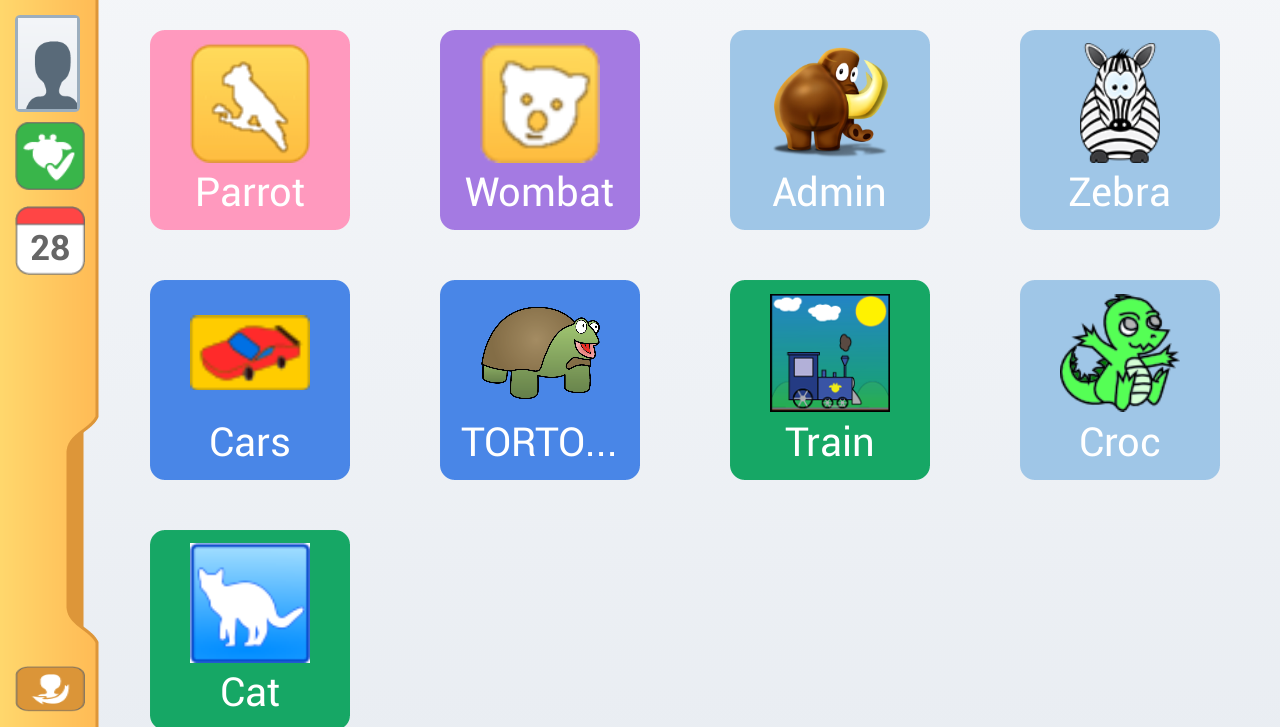
\includegraphics[width=\textwidth]{screenshots-old-giraf/giraf-homeactivity.png}
	\caption{\homeactivity.}
	\label{fig:launcheractivity:home}
	\end{subfigure}
	\begin{subfigure}[b]{.48\textwidth}
	\centering
	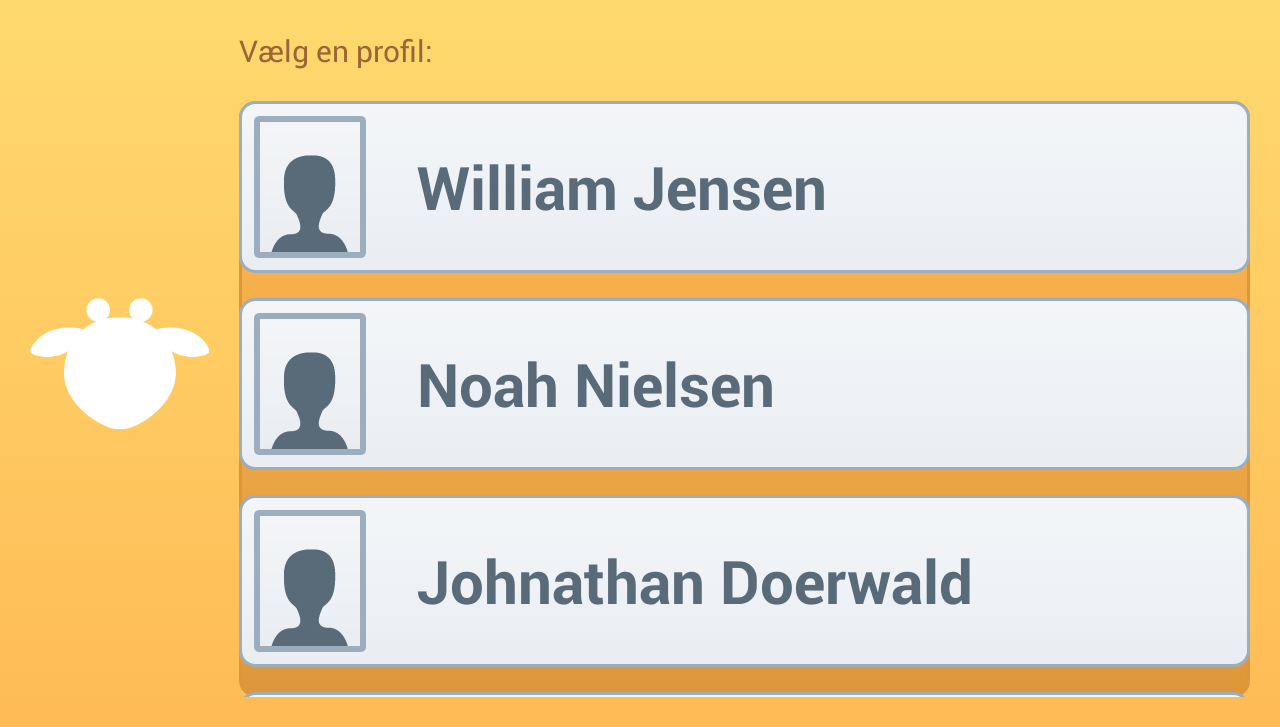
\includegraphics[width=\textwidth]{screenshots-old-giraf/giraf-profileselect.png}
	\caption{\profileselectionactivity.}
	\label{fig:launcheractivity:profile}
	\end{subfigure}
\caption{Activities of the \giraf application.}
\label{fig:launcheractivities}
\end{figure}

\paragraph{\mainactivity} is only responsible for showing the \giraf logo for a specified amount of time, as seen in \cref{fig:launcheractivity:logo}, and then redirecting the users to the proper activity.
It redirects to \authenticationactivity if the user is not logged in, or to the \homeactivity if the user is already logged in.

\paragraph{\authenticationactivity} requires the user to authenticate him- or herself before proceeding. 
\citet{launcher2012} describes why user identification is necessary, as access rights to the different \giraf applications must be able to vary between users.
The report furthermore describes how autistic citizens might have problems using a traditional user name and password system. 
Therefore, the \authenticationactivity is based on a QR-scanner, as seen in \cref{fig:launcheractivity:auth}.
Each citizen and guardian then uses a small brick printed with their personal QR-code they scan to identify themselves. 
The activity loads the user information from the database, and proceeds to \homeactivity.

\paragraph{\homeactivity} allows the user to launch \giraf applications available to his or her user profile. 
The availability of applications depends on whether the application exists locally on that device, and on whether the user is marked in the database as having proper access rights to that application.
The \homeactivity for a guardian user is seen in \cref{fig:launcheractivity:home} with the users installed \giraf applications.
Furthermore, a widget allows the user to see the synchronization status of the local database in relation to the remote database\footnote{The connection indicator widget currently has no effect, since database synchronization is not yet implemented.}, and another widget shows the current date.
There is also a widget that allows the user to log out, and return to the \authenticationactivity.
These widgets are supplied by \textit{\giraf Components}.
Finally, there is a colour palette hidden in a drawer component, where the user can change the base colour of each installed application.
The idea is to make it easier for the citizens to differentiate between the various applications by being able to choose their own colour scheme. 
Ideally, the choice of colour should also reflect in the application started from \launcher, giving the citizen consistent visual associations throughout \giraf.
The latter is for example implemented in the \textit{Tidstager} application.

\paragraph{\profileselectionactivity} is started when a guardian starts an application from \launcher. 
It displays a list of all citizens associated with this guardian, seen in \cref{fig:launcheractivity:profile}, allowing him or her to choose which citizens profile to use, when starting the selected application. 
When a citizen is logged in, the application starts, omitting the \profileselectionactivity.